\documentclass[10pt]{article}

\usepackage{graphicx}
\usepackage{amssymb}
\usepackage{amsmath}
\usepackage{ifthen}
\usepackage{epsfig}
\usepackage{fancyvrb}
\usepackage{url}
\usepackage{fancyhdr}

\usepackage{amsmath}
\usepackage{mathspec}
\usepackage{microtype}
\setmainfont[
    Numbers={Monospaced,OldStyle},
    BoldFont={Guardian TextEgyp Medium},
  ]{Guardian TextEgyp}\linespread{1.2}
\setsansfont[BoldFont={Helvetica Neue Medium}]{Helvetica Neue}\linespread{1.2}
\setmonofont[Scale=0.90]{Menlo}\linespread{1.2}
\setmathrm{Palatino}
\setmathfont(Digits,Latin,Greek){Palatino}

\tolerance=5000

\usepackage[margin=1.25in,includeheadfoot]{geometry}

\setlength{\skip\footins}{10mm}      % obsessing about footnote spacing
\setlength{\parskip}{1ex}            % paragraph spacing
\setlength{\parindent}{0ex}          % paragraph indentation

\usepackage[compact,noindentafter]{titlesec}
\titleformat*{\section}{\sffamily\large\bfseries}
\titlespacing{\section}{0pt}{2ex}{1ex}
\titleformat*{\subsection}{\sffamily\normalsize\bfseries}
\titlespacing{\subsection}{0pt}{2ex}{0ex}

% LISTS
\usepackage{enumitem}
\setenumerate{nolistsep,itemsep=1.0ex,parsep=0.0ex,leftmargin=*}
\setitemize{nolistsep,itemsep=1.0ex,parsep=0.0ex,leftmargin=*}

\usepackage[iso]{datetime}
\usdate

% ------- CUSTOM TITLE FORMAT -------
%
\makeatletter
\renewcommand{\maketitle}{
\begin{flushleft}          % right align
{\Large\sffamily\bfseries\@title}   % increase the font size of the title
\vspace{3ex}\\            % vertical space between the title and author name
{\normalsize\sffamily\@author}           % author name
\vspace{0ex}\\             % vertical space between author name and date
\normalsize\sffamily\@date                     % date
\vspace{5ex}              % vertical space between the author block and abstract
\end{flushleft}
}
% -----------------------------------

% DEFINE SOME COLORS
\usepackage{color}
\definecolor{light-blue}{RGB}{37,128,162}
\definecolor{light-gray}{gray}{0.975}
\definecolor{dark-gray}{gray}{0.50}

% CODE LISTINGS
\usepackage{listings}
\lstset{columns=fullflexible,
  basicstyle=\ttfamily\small,
  backgroundcolor=\color{light-gray},
  frame=lines, frame=lrtb, framesep=3pt, rulecolor=\color{dark-gray},
  aboveskip=10pt,
  belowskip=15pt,
  breaklines=true,
  showstringspaces=false,
  keepspaces=true,
}


\title{Assignment 6---Introduction to Statistics Using R}
\author{Paul Gribble}
\date{Winter, 2017}


\begin{document}

\maketitle

\thispagestyle{empty}

{\flushleft \sffamily * Due Friday Mar 31}

\section*{Power Calculations}

You are planning a new reaction time study. You plan
to have a main experimental condition and a control condition. The
control condition has been used previously in your lab, and when you
look at the previous data across many subjects, the reaction time data
are best characterized using an
\emph{ex-gaussian}~\footnote{\url{http://en.wikipedia.org/wiki/Exponentially_modified_Gaussian_distribution}}
distribution with the following parameters: $\mu=600$, $\sigma=60$,
$\nu=200$. Note that in \texttt{R}, the function \texttt{rexGAUS()} in
the \texttt{gamlss.dist} package can be used to generate random
samples from the ex-gaussian distribution.

\begin{center}
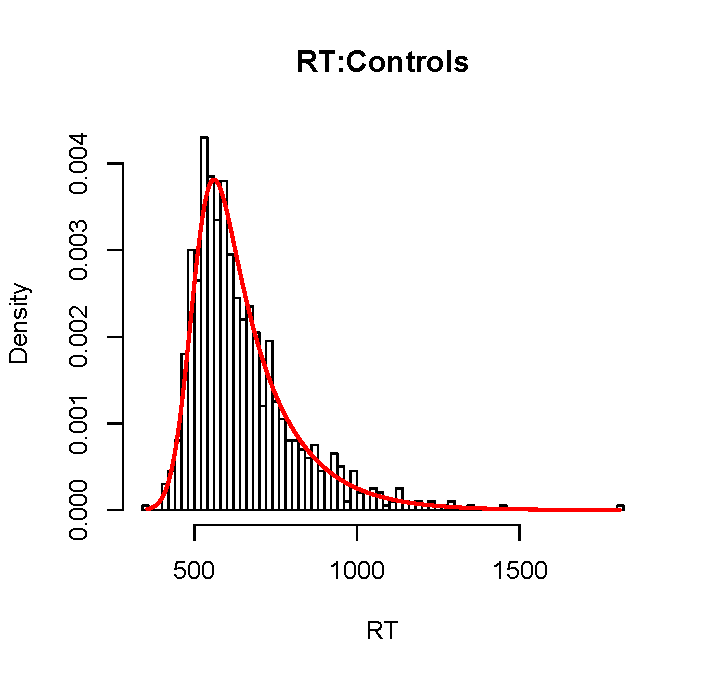
\includegraphics[height=2.5in]{RTexGaus.pdf}
\end{center}

Nobody has tried the experimental condition that you're planning, but
other studies in the literature that use reaction time as a measure
typically see changes in reaction time that correspond to a decrease
in the $\mu$ parameter of the ex-gaussian of about -50 milliseconds
(50 ms faster than controls). You plan to use a Mann-Whitney U test to
compare differences in mean reaction time between your control group
and your experimental group.

Note that the \texttt{rexGAUS()} function runs slow in R. Instead you can implement
random sampling from an ex-gaussian distribution by taking the sum of
random values from a gaussian distribution and an exponential
distribution. For example for the purposes of speed in this
assignment, you can assume that \texttt{rnorm(1000,600,60) +
  rexp(1000,1/200)} will give you 1000 random values from an
ex-gaussian distribution, just as if you were to get them using:
\texttt{rexGAUS(1000,600,60,200)}.


\begin{enumerate}
\item Use parametric bootstrapping to estimate how many subjects you
  would require in each group (assume equal group sizes) in order to
  detect a difference of -50 milliseconds at least 80\% of the time;
  in other words, to get a statistical power of 0.80. Assume an alpha
  level of 0.05.
  \item How would your answer change if you used an alpha level of 0.01?
  \item If the effect is only -25 milliseconds, how many subjects
    would you need for a power of 0.80 (using alpha 0.05)?
\end{enumerate}


\section*{Hypothesis Testing}

After running an experiment with a control group and an experimental
group, your data look like
this:~\footnote{\url{http://www.gribblelab.org/stats/data/A04data.txt}}

\begin{center}
\begin{tabular}{cc|cc}
\multicolumn{2}{c}{control} &\multicolumn{2}{c}{experimental}\\
\hline
935 &508  &857 &801\\
557 &571  &511 &772\\
607 &564  &694 &635\\
767 &713  &541 &1207\\
717 &611  &719 &663\\
515 &972  &1143 &613\\
498 &438  &680 &579\\
557 &641  &1161 &1128\\
492 &653  &837 &475\\
803 &714  &609 &883\\
\end{tabular}
\end{center}

\begin{enumerate}
\setcounter{enumi}{3}
\item Use non-parametric bootstrapping to test the null hypothesis
  that the two groups were sampled from the same population with the
  same mean.
\end{enumerate}


\end{document}

